\documentclass[25pt, a0paper, landscape]{tikzposter}
\usepackage{etstikzposter}
\usepackage{multirow}
\usetikzlibrary{arrows, decorations.markings, arrows.meta,positioning}
\usepackage{overpic}

\usepackage{sansmath}
\usepackage[sfdefault]{FiraSans}
\usepackage{amsmath, amssymb, amsthm, amsfonts}

\renewcommand{\familydefault}{\sfdefault}
\sansmath


\begin{document}
\maketitle

% Node for title, authors, and institute
\node [text=titlefgcolor,
    outer sep=0pt,
    minimum width=\textwidth,
    minimum height=8cm,
    align=center,
    fill=titlebgcolor, inner sep=1mm] at (0,11) {  % Adjust yshift as needed

\begin{minipage}[c][][c]{0.77\linewidth}
    \hspace*{30pt} 
    \fontsize{80}{90}\selectfont \textbf{Multi-person Physics-based Pose Estimation for Combat Sports}\\[12pt]
    \hspace*{30pt} 
    \fontsize{60}{80}\selectfont Hossein Feiz$^{1,*}$ \quad David Labbé$^{1}$ \quad Sheldon Andrews$^{1}$ \\[6pt]
    \hspace*{30pt} 
    \fontsize{50}{60}\selectfont $^1$École de technologie supérieure, Montréal, Québec, Canada % Adjusted font size
\end{minipage}%
\begin{minipage}[c][][c]{0.23\linewidth}
    \hspace*{-300pt}
    
\includegraphics[height=8cm]{figures/image11.png}%
    \hspace*{-10pt} % Adjust spacing between images
    
\includegraphics[height=7cm]{figures/image6.png}%
    \hspace*{-10pt} % Adjust spacing between images
    
\includegraphics[height=7cm]{figures/image5.png}%
    \hspace*{-10pt} % Adjust spacing between images
    
\includegraphics[height=7cm]{figures/image9.png}
\end{minipage}

};

\begin{columns}
    \column{0.5}
    \block{Introduction}{
        Motion capture from only RGB cameras in a typical sports scene (e.g., boxing), with the presence of coaches, viewers, and close interactions between athletes, brings many challenges, such as heavy occlusion, background crowding, and fast, complicated movements. To address this problematic, a multi-view configuration was used. Our system only required the visibility of an athlete from two cameras. We also created a pipeline using machine and deep learning techniques that automated the process of creating animations.
    }

    \block{Pipeline}{

    \begin{overpic}[scale=3]{figures/pipeline.pdf}
    \put(65,19){\fontsize{40}{16}\selectfont$L_{2D}+L_{3D}+L_{\beta}$}
    \put(0,2){\fontsize{7}{16}\selectfont$\mathrm{Y}_1$}
    \put(88,19){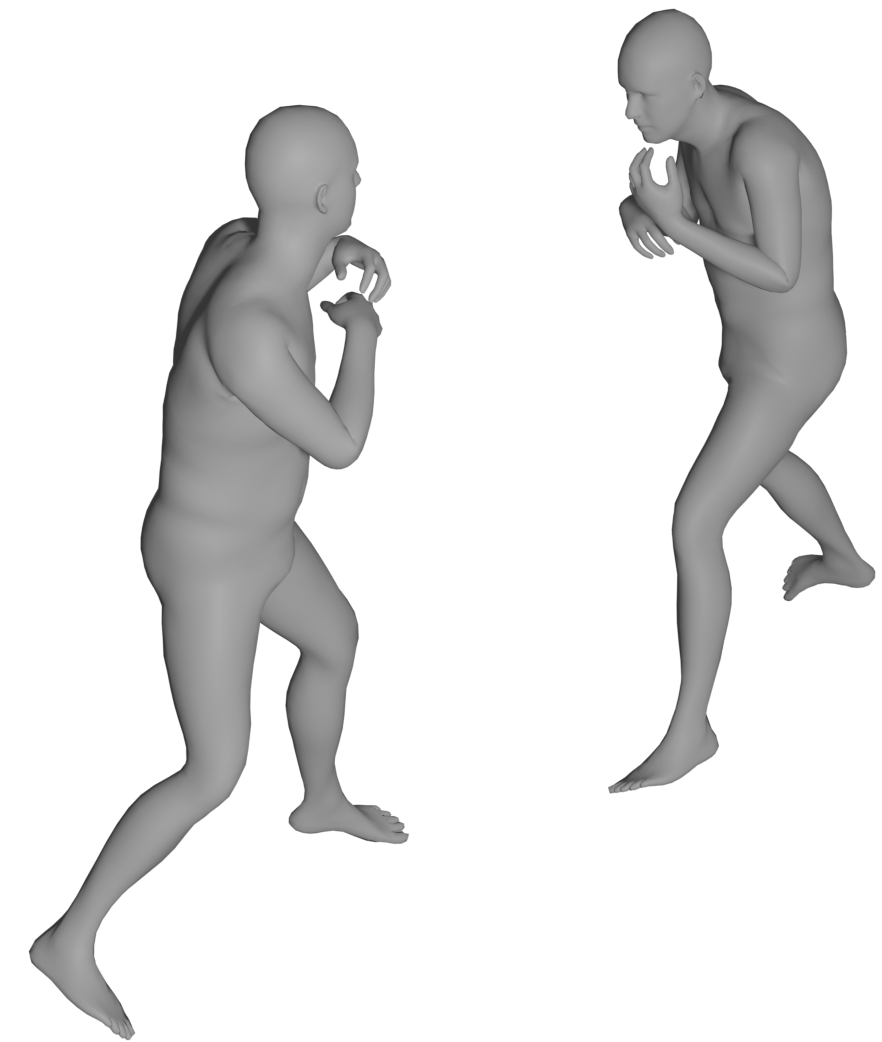
\includegraphics[scale=0.2]{figures/smpl2.png}} 
    \put(0.5,8){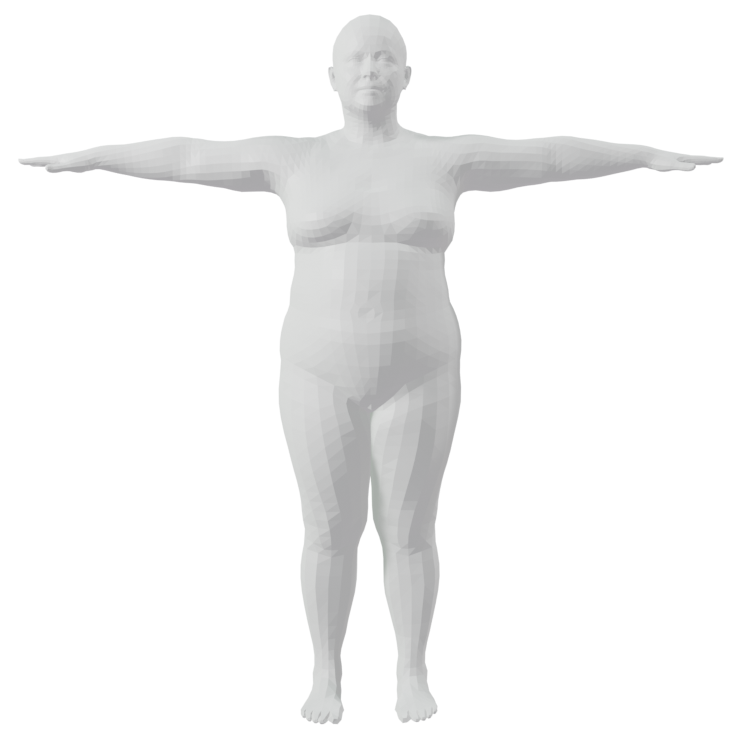
\includegraphics[scale=0.13]{figures/smpl-fat.png}} 
    \put(0,0){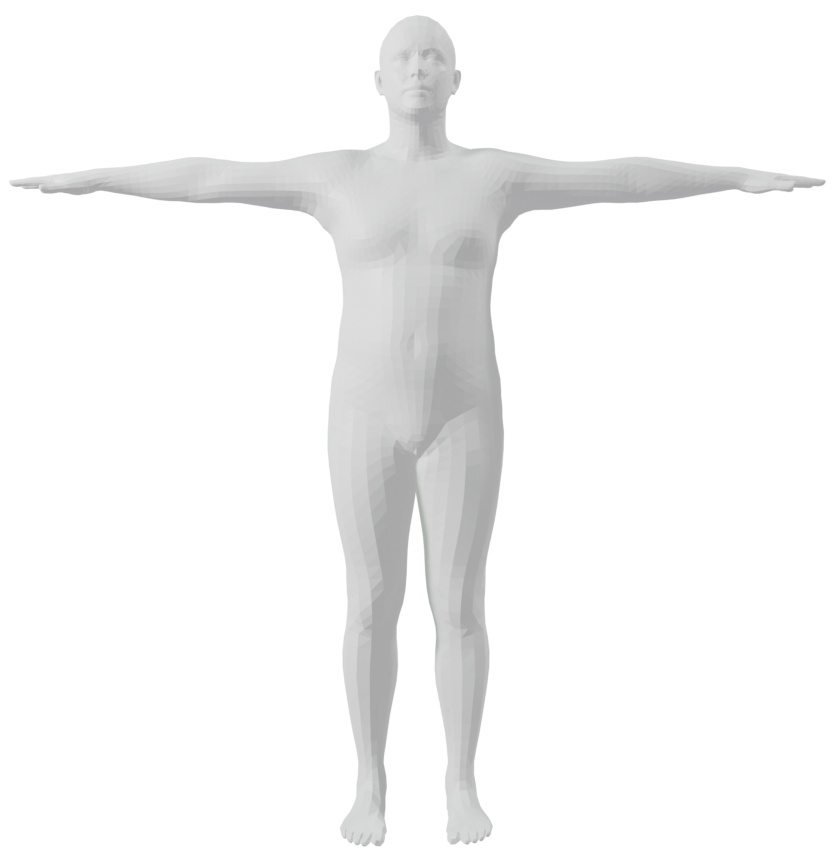
\includegraphics[scale=0.13]{figures/smpl-tall.png}}
    \put(88,19){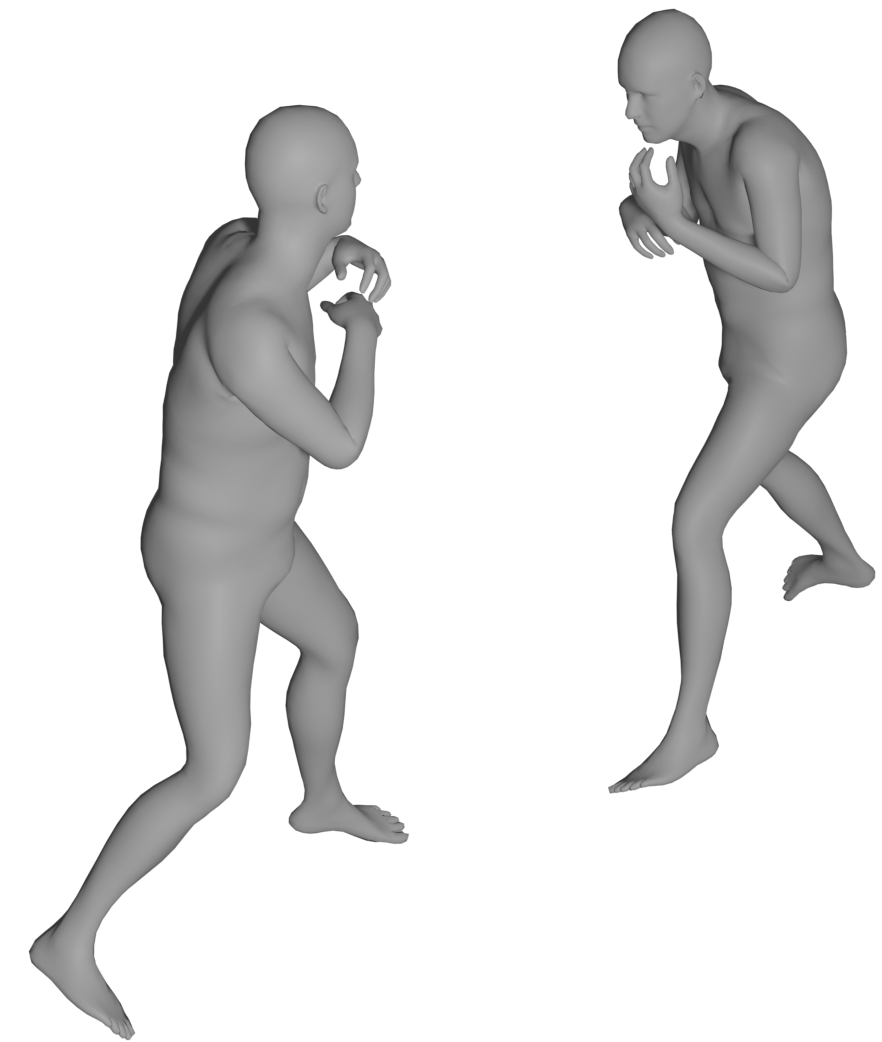
\includegraphics[scale=0.2]{figures/smpl2.png}} 
    \put(43.2,8){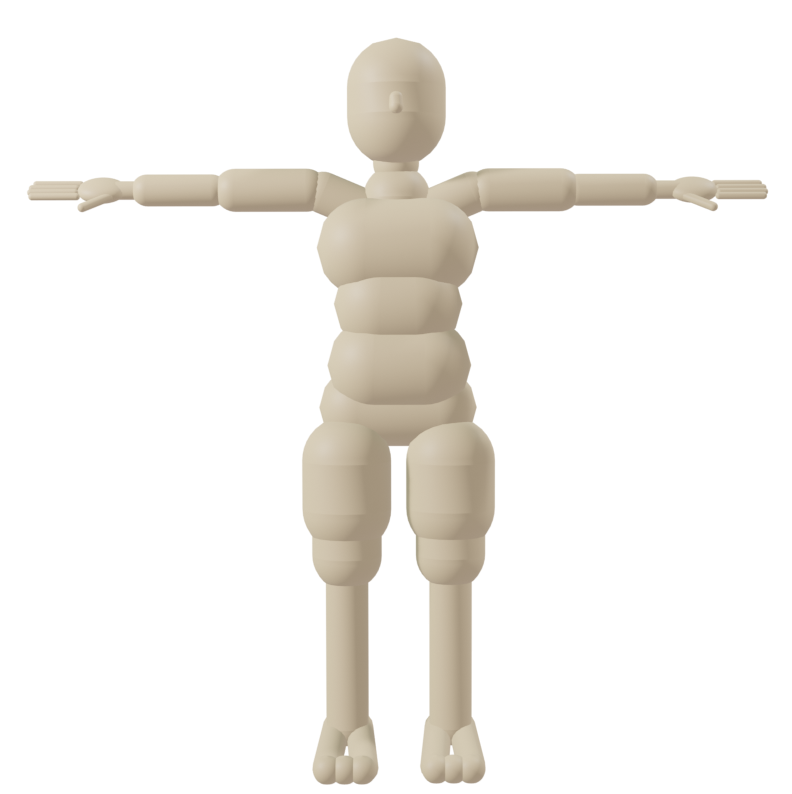
\includegraphics[scale=0.13]{figures/mujoco-fat.png}} 
    \put(43,0){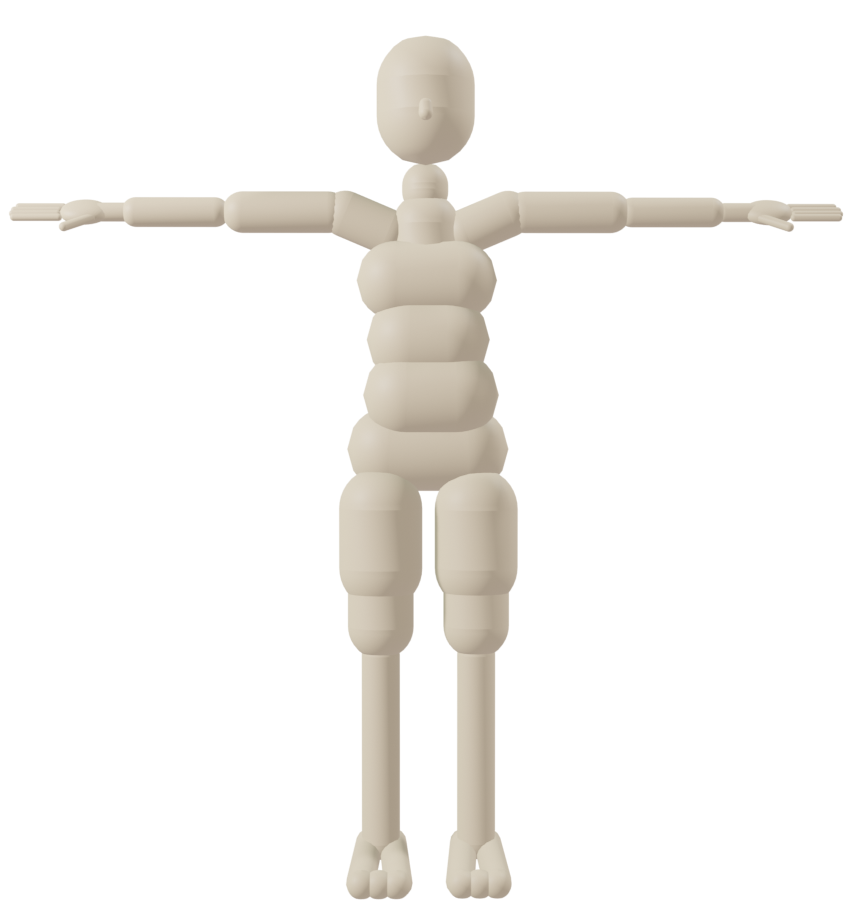
\includegraphics[scale=0.13]{figures/mujoco-tall.png}} 
    \put(88,0){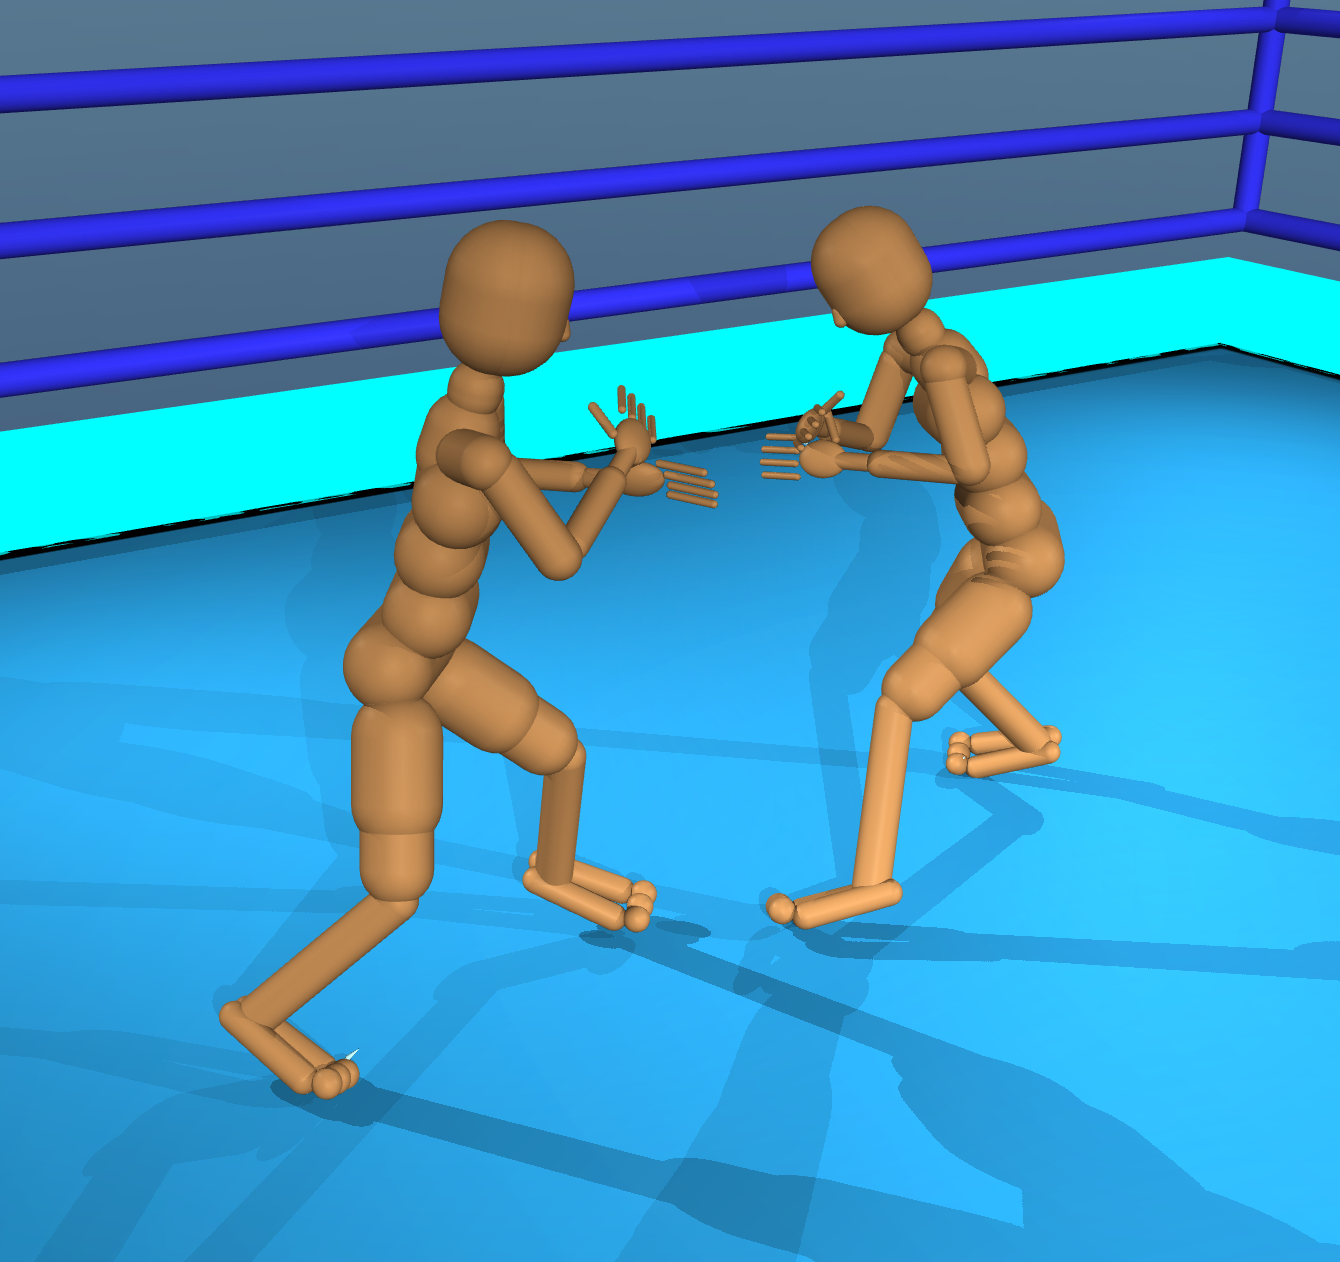
\includegraphics[scale=0.28]{figures/final.png}} 
    \end{overpic}}


    \block{Physics Body Model Generator}{
        This is the future...
        \vspace{24pt}
        \innerblock{Theorem}{
            This is a theorem
        }
    }

    \block{Weighted Triangulation and Filtering}{
The weighted triangulation estimates the 3D positions of the keypoints from their corresponding 2D keypoints from all $N$ cameras. The 3D positions of each joint are thus determined by solving the linear system:
\innerblock{Weighted Triangulation}{
\begin{tabular}{p{0.5\linewidth} p{0.45\linewidth}}
\begin{equation}
\begin{bmatrix}
\mu_{1} (\mathbf{P}_{11} - \mathrm{u}_1 \mathbf{P}_{31}) \\
\mu_{1} (\mathbf{P}_{21} - \mathrm{v}_1 \mathbf{P}_{31}) \\
\vdots \\
\mu_{N} (\mathbf{P}_{1N} - \mathrm{u}_N \mathbf{P}_{3N}) \\
\mu_{N} (\mathbf{P}_{2N} - \mathrm{v}_N \mathbf{P}_{3N}) \\
\end{bmatrix}
\begin{bmatrix}
\mathrm{x} \\
\mathrm{y} \\
\mathrm{z} \\
1
\end{bmatrix}
=
\begin{bmatrix}
0\\
\vdots \\
0
\end{bmatrix} \,,
\label{eq:tri}
\end{equation}
&
\begin{minipage}[t]{\linewidth}
$\mathbf{P}_{ij}$ extracts the $i$-th row of the projection matrix $\mathbf{P}_{j}$. $\mu_{j}$ is the average confidence of a 2D point for the current frame in camera $j$. Higher confidence values give more weight to certain cameras. We use SVD to solve Eq.~\ref{eq:tri}.
\end{minipage}
\end{tabular}
}
After triangulation, outliers are handled by interpolating and smoothing using cubic spline for each joint's trajectory. If there is no solution for triangulation, we utilize an extended Kalman filter for dynamic state estimation based on velocity, acceleration of the keypoint, and position constraint to estimate the 3D keypoints. This results in robust filtering and smoothing while preserving trajectory integrity, enabling dependable 3D reconstructions from sparse and noisy 2D keypoints.
}

        
    \column{0.5}
    \block{Multi-frame Multi-view Tracking IDs}{
        \begin{minipage}{0.6\linewidth}
            \begin{itemize}
                \item 1st item on the right
                \item 2nd item on the right
                \item 3rd item on the right
            \end{itemize}
        \end{minipage}
        \begin{center}
            \hspace{2cm}
        \end{center}
        \innerblock{An Inner Block}{
            Say something important here
        }
        \begin{equation}
            E = mc^2 
        \end{equation}
        \begin{equation}
            a \in \mathbb{R}^n
        \end{equation}
    }

\end{columns}

% Node for images at the bottom of the poster
\node [above right,
    text=titlefgcolor,
    outer sep=0pt,
    minimum width=\textwidth,
    minimum height=2cm,
    align=left,
    fill=titlebgcolor,inner sep=1mm] at (bottomleft) {


};
\end{document}